\documentclass[twoside,a4paper]{refart}
\usepackage{makeidx}
\usepackage{ifthen}
%\usepackage{geometry}
%\usepackage{ngerman}
\usepackage{longtable}
\usepackage[T1]{fontenc}
\usepackage{ae}
\usepackage[utf8]{inputenc}
\usepackage{fancyhdr}
\usepackage{graphicx}
\usepackage{xspace}
\usepackage[cmyk]{xcolor}
\usepackage{amsmath}
\usepackage[
  %plainpages=false,
  %pdfpagelabels,
  %colorlinks=true,
  pdfborder={0 0 0},
  %urlcolor=blue,
  %linkcolor=blue,
  bookmarksopen=true,
  %pdfstartpage=3,
  unicode,
]{hyperref}
\hypersetup{
  pdftitle={CodeCover - Manual},
  pdfsubject={CodeCover - Manual},
  pdfauthor={Stefan Franke, Robert Hanussek, Benjamin Keil, Steffen Kieß, Johannes Langauf, Christoph Marian Müller, Igor Podolskiy, Tilmann Scheller, Michael Starzmann, Markus Wittlinger},
  pdfkeywords={CodeCover, Manual},
}
% hypcap is needed for correct links to figures, see specification Bug 2
\usepackage[all]{hypcap}
\usepackage{svnkw}
\usepackage[USenglish]{isodate}
\usepackage{titlesec}
% provides \ul,  allows line breaking for underlined text (static methods...)
\usepackage{listings} % for the source code in the tex document
\lstset{numbers=left,%
        numberstyle=\small,%
        keywordstyle=\textbf,%
        numbersep=5pt}
\usepackage{soul}
\makeatletter

% some TeX voodoo to extract the date from SVN ID
% which can be processed by isodate 
\def\svn@dateonly#1 #2Z{#1}
\def\svndateonly#1{%
\ifx#1\empty1970-01-01\else
\expandafter\svn@dateonly#1\fi}

% Two-level figure & table numbering
\@addtoreset{table}{section}
\@addtoreset{figure}{section}
\renewcommand{\thefigure}{\thesection.\arabic{figure}}
\renewcommand{\thetable}{\thesection.\arabic{table}}
\makeatother

% custom font sizes for headings, non run-in titles for [sub]paragraphs
\titleformat{\section}{\bfseries\fontsize{24}{30}\selectfont\sffamily}{\thesection}{1em}{}
\titleformat{\subsection}{\bfseries\fontsize{18}{24}\selectfont\sffamily}{\thesubsection}{1em}{}
\titleformat{\subsubsection}{\bfseries\fontsize{16}{22}\selectfont\sffamily}{\thesubsubsection}{1em}{}
\titleformat{\paragraph}{\bfseries\fontsize{14}{20}\selectfont\sffamily}{\theparagraph}{1em}{}
\titleformat{\subparagraph}{\bfseries\normalsize\sffamily}{\thesubparagraph}{1em}{}
\titlespacing{\paragraph}{0pt}{\parskip}{-0.5\parskip}{}
\titlespacing{\subparagraph}{0pt}{\parskip}{-0.5\parskip}{}

\svnid{$Id: Manual.tex 1 2007-12-12 17:37:26Z t-scheller $}

\parindent0mm
\parskip2mm
%\geometry{textwidth=160mm, textheight=230mm, inner=30mm}

\xdefinecolor{TodoColor}{rgb}{1.0, 0.0, 0.0}

% depth of the headlines that are numbered
\setcounter{secnumdepth}{5}
\setcounter{tocdepth}{5}

\newcommand{\OSTWeST}{\textit{OSTWeST}\xspace}
\newcommand{\codecover}{\textit{CodeCover}\xspace}
\newcommand{\software}{\textit{DeepThought}\xspace}
\newcommand{\eclui}{\textsf}
\newcommand{\code}{\texttt}
\newcommand{\todo}[1]{\bgroup\color{TodoColor}\textsc{\textbf{TODO:} #1}\egroup}
\newcommand{\BIG}{\fontsize{48}{48}\selectfont}
\newcommand{\linkwithfootnote}[2]{\href{#1}{#2}\footnote{\url{#1}}}
\newcommand{\email}[1]{\href{mailto:#1}{#1}}

\xdefinecolor{ClassColor}         {rgb}{0.0, 1.0, 0.0}
\xdefinecolor{ClassAbstractColor} {rgb}{0.0, 1.0, 0.0}
\xdefinecolor{ObjectColor}        {rgb}{0.31, 0.58, 0.84}
\xdefinecolor{InterfaceColor}     {rgb}{1.0, 0.0, 1.0} % that's magenta NOT pink, OK? ;-)
\xdefinecolor{ImplementerColor}   {rgb}{0.4, 0.2, 0.6}
\xdefinecolor{FieldColor}         {rgb}{0.9, 0.5, 0.0}

\newcommand{\pkg}[1]{\texttt{#1}}
\newcommand{\cls}[1]{\texorpdfstring{{\color{ClassColor}\texttt{#1}}}{#1}}
\newcommand{\clsab}[1]{\texorpdfstring{{\color{ClassAbstractColor}\textit{\texttt{#1}}}}{#1}}
\newcommand{\obj}[1]{\texorpdfstring{{\color{ObjectColor}\texttt{#1}}}{#1}}
\newcommand{\itf}[1]{\texorpdfstring{{\color{InterfaceColor}\texttt{#1}}}{#1}}
\newcommand{\imp}[1]{\texorpdfstring{{\color{ImplementerColor}\texttt{#1}}}{#1}}
\newcommand{\mtd}[1]{\texttt{#1}}
\newcommand{\mtdst}[1]{\texorpdfstring{\ul{\texttt{#1}}}{#1}}
\newcommand{\mtdab}[1]{\texorpdfstring{\textit{\texttt{{#1}}}}{#1}}
\newcommand{\fld}[1]{{\color{FieldColor}\texttt{#1}}}
\newcommand{\namespace}[1]{\begin{description}\item[Namespace:]#1\end{description}}
\newcommand{\rootpkg}{org.gbt2}

\newcommand{\codepageflag}{iscodecontainer}

% needed for the Function Point tables
\newcommand{\x}{\textbullet}

%\includeonly{Introduction}
%\includeonly{UserInterface}
%\includeonly{FunctionalRequirements}
%\includeonly{NonFunctionalRequirements}
%\includeonly{Conclusion}
\begin{document}

% --- title page --- %
\pagestyle{empty}
\begin{fullpage}
\begin{titlepage}
 \vspace*{38mm}
 \begin{center}
 \fontsize{24}{24}\selectfont
 User's Manual\\
 \vspace*{12mm}
 \fontsize{48}{48}\selectfont
 
 % gross hack to generate the a big fancy gbt-squared appearance
 \textit{CodeCover}
 %
 \\
 \fontfamily{\familydefault}\fontsize{32}{38}\selectfont
 Glass Box Testing Tool\\
 \vspace*{12mm}
 \fontsize{16}{20}\selectfont
 Student Project A ``OST-WeST''\\
 University of Stuttgart

 \vspace{2cm}
 {\small 
   Version: 1.0 Beta \\
   {Last changed on \printdate{\svndateonly{\svndate}} (SVN Revision \svnrev)}}
   \end{center}
   \vspace{3cm}
   \hspace{40mm}
   \normalsize
\end{titlepage}
\end{fullpage}

% --- Header and version history --- %

\cleardoublepage
\fancyhf{}
\fancyhead[LO,RE]{\textit{\codecover\ -- User's Manual}}
\fancyhead[LE,RO]{\thepage}
\pagestyle{fancyplain}

% --- Table of contents --- %

\parskip1mm
\tableofcontents
\parskip2mm

\pagestyle{fancyplain}
\renewcommand{\baselinestretch}{1.25}\normalsize
\svnid{$Id: Introduction.tex 1 2007-12-12 17:37:26Z t-scheller $}
\section{Introduction} \label{Introduction}

\subsection{Project overview} \label{in:Overview}
\gbt is a glass box testing tool to measure the coverage of a running program.
It will be as independent as possible of the programming language of the covered program.

%TODO: Bla Bla bla...
\subsection{About this document} \label{in:AboutThisDocument}

This document contains the necessary information to create a detailed design
obeying the requirements documented in the specification. It describes the
behaviour of the software and the artifacts which are created by it. The
architecture is also defined by this document, as well as the data structures
used to store the data pertaining to the operation of the software. Details
like the structure of classes and the design of methods have to be determined
in the detailed design document.


\subsection{Addressed audience} \label{in:Addressed audience}
This document is addressed to
\begin{itemize}
  \item the customer who ordered the software
  \item the project manager controlling the work
  \item the quality assurance division creating test cases for the software
  \item the developers implementing the design
  \item future developers maintaining and extending the software
  \item interested users of the software
  \item students of upcoming student projects
\end{itemize}

\subsection{Authors}
In the following table authors of this document are named.
{\small
\begin{longtable}{|p{35mm}|p{65mm}|l|} \hline
   {\normalsize \textbf{Author}} &
   {\normalsize \textbf{E-mail}} \\\hline \hline \endhead
   Robert Hanussek & \email{hanussrt@studi.informatik.uni-stuttgart.de} \\\hline
   Steffen Kieß & \email{kiesssn@studi.informatik.uni-stuttgart.de} \\\hline
   Tilmann Scheller & \email{schellrt@studi.informatik.uni-stuttgart.de} \\\hline
   Markus Wittlinger & \email{wittlims@studi.informatik.uni-stuttgart.de} \\\hline
\end{longtable}
}




\subsection{Notation}

\subsubsection{Identifiers}

\cls{FooBar} denotes a class named \code{FooBar}.

\clsab{FooBar} denotes an abstract class named \code{FooBar}.

\obj{FooBar} denotes an instantiated object of class \cls{FooBar}.

\itf{FooBar} denotes an interface class named \code{FooBar}.

\imp{FooBar} denotes an object of a class which implementes the interface named \code{FooBar}.

\mtd{fooBar(...)} denotes a method named \code{fooBar} which has parameters (which are not listed). Methods don't have a special color because they can be easily identified by the trailing brackets.

\mtd{fooBar()} denotes a method named \code{fooBar} which doesn't have any parameters.

\mtdst{fooBar(...)} denotes a static method (which has parameters).

\fld{fooBar} denotes a field named \code{fooBar}.

\pkg{foo.bar} denotes a package called \code{bar} which resides in a package called \code{foo}. Packages don't have a special color because they can be identified easily since they are the only items which contain a dot and are lower case.

%% \subsubsection{Namespace}

%% Every section can define a namespace. All relative paths in such a section are relative to this namespace except paths which point to standard Java classes which are listed below. If for example the namespace \pkg{\rootpkg.report} is defined then \pkg{html.}\cls{Report} points to class \cls{Report} which resides in the package \pkg{\rootpkg.report.html}. It is also possible to define namespaces which refer to classes, e.g. \pkg{\rootpkg.report.}\cls{Report}. This allows it to directly reference the methods in \cls{Report} (see~\ref{Classes:Report:Report} for an example).

%% Namespaces are defined directly under the header of a section and are valid for the section the header belongs to. A Namespace definition looks like this:
%% \namespace{\pkg{\rootpkg.report}}

%% Following standard Java classes are used in this document without specifing their fully qualified package paths. These classes are also unaffected by namespace definitions:
%% % we will just write String instead of java.lang.String
%% \begin{itemize}
%% \item \pkg{java.lang.}\cls{String}
%% \item \pkg{java.io.}\cls{OutputStream}
%% \item \pkg{java.util.}\itf{List}
%% \end{itemize}

\svnid{$Id: Quickstart.tex 1 2007-12-12 17:37:26Z t-scheller $}
\section{Quickstart Guide}\label{qsg}
This section provides you, the aspiring \codecover user, with a step by step instruction set, that, starting with a piece of software, progressing over the instrumentation, compilation of the instrumented software, and its execution, results in an html-report, containing the coverage data measured during the execution. 
\subsection{General Preconditions}
\begin{itemize}
\item The name of the software used in this example is \software
\item \software is written in Java
\item \software sources are encoded using UTF-8
\item \codecover is executed with the \code{codecover} command
\item \verb$CODECOVER_HOME$ refers to the installation directory of \codecover
\end{itemize}

\subsection{Instrument}
The first step lies in the instrumentation of \software with the following command: 
\begin{verbatim}
codecover instrument
    --root-directory DeepThought/src
    --destination DeepThought/instrumentedSrc 
    --container DeepThought/test-session-container.xml
    --language java 
    --charset UTF-8 
\end{verbatim}
\begin{itemize}
\item The option \code{root-directory} refers to the directory of the software, that holds the top-level package(s) of the to be instrumented code.
\item The option \code{destination} refers to the directory the instrumented source files are put.
\item The option \code{container} refers to the test session container, that holds the static information about the instrumented code, as well as the later the collected coverage data.
\item The option \code{language} refers to the language of the to be instrumented code, which in this case equates to Java.
\item The option \code{charset} refers to the charset, in which the source files are saved in.
\end{itemize}

You will commence the instrumentation process with the execution of this command, whose duration depends on the size of the to be instrumented code. As a result of said process a number of new, instrumented source files are created in the specified destination.

\subsection{Compile}
After the instrumentation of the software follows now the compilation of the instrumented source code. This falls outside the purview of \codecover and your job. It must be noted, that any additional source files created by \codecover must be compiled alongside the instrumented source code.

\subsection{Execute}
You can now execute the compiled program, which will result in a coverage log file. This file holds, for now, the coverage data measured during the execution and, in the next step, will be entered into the test session container.

\subsection{Analyze}
The created coverage log file is entered into the test session container with the following command:
\begin{verbatim}
codecover analyse 
    --container DeepThought/test-session-container.xml 
    --coverage-log DeepThought/coverage_log.clf 
    --name TestSession1 
    --comment "The first test session"
\end{verbatim}
\begin{itemize}
\item The option \code{container} refers to the test session container, into which the coverage data is to be entered, ordinarily the test session container created during the instrumentation process. 
\item The option \code{coverage-log} refers to the coverage log file, whose coverage data is to be entered into the test session container.
\item The option \code{name} refers to the name of the test session, the coverage data is attributed to.
\item The option \code{comment} refers to an optional comment, that can be added to a test session.
\end{itemize}
You will enter the coverage data of the coverage log file into the test session container with the execution of this command. The coverage log file is no longer needed after the successful completion of the command.

\subsection{Interlude}
You can now repeat the execution of the software and the analyzing of the resulting coverage log into further test sessions. Since the report can currently be based only on a single test session, provides \codecover you with a command, that can merge existing test sessions into a single test session, that contains all the data of the precursor test sessions. If you didn't create multiple test sessions, or don't want to merge the test sessions, then you can skip the following step and continue on to the creation of the report.

\subsection{Merge test sessions}
Multiple test sessions can be merged into a single test session, with the following command:
\begin{verbatim}
codecover merge-sessions 
    --container DeepThought/test-session-container.xml 
    --sessions TestSession1 
    --sessions TestSession2 
    --name "TestSession1+2" 
    --comment "TestSession1 and TestSession2" 
\end{verbatim}
\begin{itemize}
\item The option \code{container} refers to the test session container, which holds the to be merged test sessions.
\item The option \code{sessions} refers to individual test sessions, that are to be merged. It is assumed here, that you created a second test session with the name "TestSession2".
\item The option \code{name} refers to the name of the merged test session
\item The option \code{comment} refers to an optional comment, that can be added to the merged test session.
\end{itemize}
Execution of this command creates a new test session with the name "TestSession1+2", that holds all the coverage data of the precursor test sessions.

\subsection{Generate Report}
Finally \codecover can generate a report of one of the test sessions in the test session container with the following command:
\begin{verbatim}
codecover report 
    --container DeepThought/test-session-container.xml 
    --destination DeepThought/report/index.html 
    --session "TestSession1+2" 
    --template CODECOVER_HOME/report-templates/HTML_Report_hierarchic.xml 
\end{verbatim}

\begin{itemize}
\item The option \code{container} refers to the test session container, which holds the test session, from which a report is generated.
\item The option \code{destination} refers to the directory, in which the report is generated and the top-level html-file of the report. At the moment, this directory must exists prior to the execution of this command.
\item The option \code{session} refers to the name of the test session, from which a report is generated. In this case it is assumed, that you merged two test sessions into the given one. Was this not the case, simply substitute the name of the test session with one of a test session you want to generate a report about.
\item The option \code{template} refers to the template used in the generation of the report.
\end{itemize}
Execution of this command will generate a report, of the given test session, at the specified location, for you to examine and concludes this guide.
\svnid{$Id: Batch.tex 1 2007-12-12 17:37:26Z t-scheller $}
\section{Command Line Interface}
\subsection{Command overview} \label{fr:Batch interface-Command overview}
For almost every command, either a long or a short version can be used. These commands can be used by \code{codecover \%\textbf{command}\% [\%options\%]}.
\begin{longtable}{|l|p{6cm}|}\hline
   {\textbf{Command}} &
   {\textbf{Description}} \\\hline \hline \endhead
   \ref{Command-Instrumenter-Info}: {ii, instrumenter-info} & get information of all available instrumenters \\\hline
   \ref{Command-Instrument}: {in, instrument} & instrumentation of code files \\\hline
   \ref{Command-Analyze}: {an, analyze} & Analysis of a coverage run to create a test-session \\\hline
   \ref{Command-Report}: {re, report} & Generating a report from a test-session \\\hline
   \ref{Command-Info}: {info} & Showing the information of a test-session container and the contained test-sessions and test cases \\\hline
   \ref{Command-Merge-Sessions}: {ms, merge-sessions} & Merging two or more test-sessions \\\hline
   \ref{Command-Alter-Session}: {as, alter-session} & Altering test-session information \\\hline
   \ref{Command-Copy-Sessions}: {cs, copy-sessions} & Copy test-sessions from one session container to another \\\hline
   \ref{Command-Remove-Sessions}: {rs, remove-sessions} & Removing test-sessions from a session container \\\hline
   \ref{Command-Merge-Test-Cases}: {mt, merge-test-cases} & Merging two or more test cases \\\hline
   \ref{Command-Alter-Test-Case}: {at, alter-test-case} & Editing test case information \\\hline
   \ref{Command-Remove-Test-Cases}: {rt, remove-test-cases} & Removing test cases from a session container \\\hline
   \ref{Command-Help}: {h, help} & A help page containing this command overview or an option and parameter overview a given command. \\\hline

  \caption{Command line interface command overview}
  \label{CLI command overview}
\end{longtable}

%%%%%%%%%%%%%%%%%%%%%%%%%%%%%%%%%%%%%
%%%%%%%%%%%%  General Commands  %%%%%
%%%%%%%%%%%%%%%%%%%%%%%%%%%%%%%%%%%%%
\subsection{General Commands}\label{General}
For every command a set of options is supported. In addition to specific command options, all commands support some global parameterless options. They are not required but change the behavior of the software when used. These commands can be used by \code{codecover \%command\% [\%\textbf{options}\%]}.
\begin{longtable}{|l|p{8cm}|}\hline
   {\textbf{Option}} &
   {\textbf{Explanation}} \\\hline \hline \endhead
     \verb$-v, --verbose$ & Orders the software to print more information as usual. For example this can be a description of the actions being done. This option is the opposite of \verb$--quiet$. \\\hline
     \verb$-q, --quiet$ & Orders the software not to print information to the shell. This option is the opposite to \verb$--verbose$. \\\hline
     \verb$-p, --pretend$ & Orders the software not to perform any actions affecting the data persistently but to print information about what the software would do instead. Using \verb$--pretend$ the actor can make sure that his command has the correct syntax and would be successfully executed. \\\hline
     \verb$-h, --help$ & Prints an option and parameter overview of the given command. Has the same effect like \verb$codecover help \%command\%$. \\\hline
     \verb$-V, --version$ & Prints out the version of the software. Has the same effect like \verb$codecover --version$. \\\hline
  \caption{General batch options}
  \label{fr_tb:General batch command options}
\end{longtable}

%%%%%%%%%%%%%%%%%%%%%%%%%%%%%%%%%%%%%
%%%%%%%%  Instrumenter-Info %%%%%%%%%
%%%%%%%%%%%%%%%%%%%%%%%%%%%%%%%%%%%%%
\subsection{Instrumenter-Info}\label{Command-Instrumenter-Info}
This command is used to get information of all available instrumenters. If there are two or more instrumenters available for a given programming language, you can get to know the unique keys of the possible instrumenters. These key can than be used for the option \code{instrumenter} of the instrument command (\ref{Command-Instrument}).

\subsubsection{Usage}\label{command:ii:usage}
\begin{quote}
\code{codecover (instrumenter-info|ii) [options]}
\end{quote}

\subsubsection{Options}\label{command:ii:options}
\seealso{\nameref{General}}
The following table lists all the options, that are available for use with this command.
%\begin{maxipage}
\begin{longtable}{|l|p{4cm}|}\hline
   {\textbf{Option}} & 
   {\textbf{Description}} \\\hline \hline \endhead
   \verb$-l, --language <lang>$ & (\code{java}|\code{cobol}) \\\hline
  \caption{Options for command instrumenter-info}
  \label{fr_tb:Options for command instrumenter-info}
\end{longtable}

\subsubsection{Examples}\label{command:ii:examples}
\begin{quote}
\begin{verbatim}
codecover instrumenter-info -l java
                            -v
\end{verbatim}
\end{quote}
Print out verbose information of all instrumenters, that support the programming language java.

%%%%%%%%%%%%%%%%%%%%%%%%%%%%%%%%%%%%%
%%%%%%%%%%%%  Instrument %%%%%%%%%%%%
%%%%%%%%%%%%%%%%%%%%%%%%%%%%%%%%%%%%%
\subsection{Instrument}\label{Command-Instrument}
This command is used to instrument source code files so that the coverage will be measured when these files will be executed.
\subsubsection{Usage}\label{command:in:usage}
\begin{quote}
\code{codecover (instrument|in) [options]}
\end{quote}

\subsubsection{Options}\label{command:in:options}
\seealso{\nameref{General}}
The following table lists all the options, that are available for use with this command.
%\begin{maxipage}
\begin{longtable}{|l|p{4cm}|c|}\hline
   {\textbf{Option}} & 
   {\textbf{Description}} & 
   {\textbf{Required}} \\\hline \hline \endhead
   \verb$-r, --root-directory <dir>$ & the root directory of the source files & \x \\\hline
   \verb$-i, --include <pattern>$ & a relative include pattern; this argument can occur more than one time &  \\\hline
   \verb$-f, --includes-file <file>$ & a file containing a list of relative include patterns separated by new line & \\\hline
   \verb$-e, --exclude <pattern>$ & a relative exclude pattern; this argument can occur more than one time & \\\hline
   \verb$-x, --excludes-file <file>$ & a file containing a list of relative exclude patterns separated by new line & \\\hline
   \verb$-o, --criterion <crit>$ & one of (\code{all}, \code{st}, \code{br}, \code{co}, \code{lo}); this argument can occur more than one time -- once for every criterion & \\\hline
   \verb$-l, --language <lang>$ & (\code{java}|\code{cobol}) & \x \\\hline
   \verb$-I, --instrumenter <key>$ & the unique key of the instrumenter to use; use the command \code{instrumenter-info} (\ref{Command-Instrumenter-Info}) to get the correct key & \\\hline
   \verb$-d, --destination <dir>$ & the destination directory for the instrumented files & \x \\\hline
   \verb$-c, --container <file>$ & the new session container & \x \\\hline
   \verb$-a, --charset <charset>$ & the character encoding of the source files & \\\hline
   \verb$-u, --copy-uninstrumented$ & advices the software to copy all files of the root-directory, that where not instrumented, to the destination & \\\hline
   \verb$-D, --directive$ & arguments of the style \code{key=value} to enable special features of the instrumenter; the instrumenter-info command prints out a list of directives, an instrumenter supports  & \\\hline
  \caption{Options for command instrument}
  \label{fr_tb:Options for command instrument}
\end{longtable}
%\end{maxipage}

The arguments of option \code{criteria} stand for:
\begin{longtable}{|c|l|}\hline
   {\textbf{Criteria abbreviation}} &
   {\textbf{Explanation}} \\\hline \hline \endhead
     \code{all} & all criteria \\\hline
     \code{st} & statement coverage \\\hline
     \code{br} & branch coverage \\\hline
     \code{co} & condition coverage \\\hline
     \code{lo} & loop coverage \\\hline
  \caption{Explanation of the criteria abbreviations}
  \label{fr_tb:Explanation of the criteria abbreviations}
\end{longtable}

\subsubsection{Patterns}
For a more detailed selection, include and exclude patterns can be used. These patterns allow wildcards and are adopted from the \linkwithfootnote{http://ant.apache.org/}{apache ant project} (see their  \linkwithfootnote{http://ant.apache.org/manual/dirtasks.html}{pattern description}).
\par
The wildcard \code{?} matches one character. The wildcard \code{*} matches zero or more characters. Examples:
\begin{itemize}
\item \code{?.java} matches  \code{x.java} and \code{A.java}, but not \code{.java} or \code{xyz.java} (both don't have one character before \code{.java}).
\item \code{*.java}  matches \code{.java}, \code{x.java} and \code{FooBar.java}, but not \code{FooBar.xml} (does not end with \code{.java}).
\end{itemize}
Combinations of \code{*}'s and \code{?}'s are allowed.
\par
To match a complete directory tree, or a file anywhere in the directory tree, use \code{**}. When \code{**} is used as the name of a directory in the pattern, it matches zero or more directories. Example:
\begin{itemize}
\item \code{src/**/*.java} matches all java files under \code{src/}, such as \code{src/x.java}, or \code{src/foo/bar/MyObject.java}, but not \code{Main.java} or \code {test/AllTests.java} (Do not lie under \code{test}).
\end{itemize}
\par
The instrumenter uses some ignore patterns for files, that are totally ignored:
\begin{itemize}
\item \verb$**/*~, **/#*#, **/.#*, **/%*%", **/._*"$
\item \verb$**/.svn/**, **/_svn/**, **/CVS/**, **/.cvsignore$
\item \verb$**/SCCS/**, **/vssver.scc, **/.DS_Store, **/Thumbs.db$
\end{itemize}

\subsubsection{Examples}\label{command:in:examples}
\begin{quote}
\begin{verbatim}
codecover instrument -r src/ 
                     -d bin/instr/ 
                     -c container.xml 
                     -l java
\end{verbatim}
\end{quote}
Find all java source files in the directory "src", parse and instrument these files into the directory "bin/instr/". The source files are instrumented for all criteria and the static information compiled during the instrumentation is stored in the "container.xml".  
\begin{quote}
\begin{verbatim}
codecover instrument -r src/ 
                     -d bin/instr/ 
                     -i "org/pak1/**"
                     -e "**/*Test.java"
                     -c container.xml 
                     -l java
                     -I CodeCover_Java_1.5
                     -o st lo
                     -a UTF-8
                     -u
\end{verbatim}
\end{quote}
Find all java source files under the directory "org/pak1", exclude files ending with "Test.java", parse these files with the "UTF-8" charset and instrument them into the directory "bin/instr/". The source files are instrumented for statement and loop coverage, and the static information compiled during the instrumentation is stored in the "container.xml". All files under "src", which are not instrumented, are copied to "bin/instr/". The code cover instrumenter for java is used. It is specified by its unique key \textit{CodeCover\_Java\_1.5}.


%%%%%%%%%%%%%%%%%%%%%%%%%%%%%%%%%%%%%
%%%%%%%%%%%%%% Analyze %%%%%%%%%%%%%%
%%%%%%%%%%%%%%%%%%%%%%%%%%%%%%%%%%%%%
\subsection{Analyze}\label{Command-Analyze}
This command is used to import a coverage-log, that was produced by an instrumented program, into a specified test-session container.
\subsubsection{Usage}\label{command:an:usage}
\begin{quote}
\code{codecover (analyze|an) [options]}
\end{quote}

\subsubsection{Options}\label{command:an:options}
\seealso{\nameref{General}}
The following table lists all the options, that are available for use with this command.
\begin{longtable}{|l|p{4cm}|c|}\hline
   {\textbf{Option}} & 
   {\textbf{Description}} & 
   {\textbf{Required}} \\\hline \hline \endhead
   \verb$-c, --container <file>$ & the test-session container the coverage data should be added to & \x \\\hline
   \verb$-g, --coverage-log <file>$ & the coverage log produced by the executed program & \x  \\\hline
   \verb$-n, --name <name>$ & the name of the new test-session containing the coverage results & \x \\\hline
   \verb$-m, --comment <text>$ & a comment describing the test-session & \\\hline
   \verb$-a, --charset <charset>$ & the character encoding of the coverage log file & \\\hline
  \caption{Options for command analyze}
  \label{fr_tb:Options for command analyze}
\end{longtable}

\subsubsection{Examples}\label{command:an:examples}
\begin{quote}
\begin{verbatim}
codecover analyze -c container.xml
                  -g coverageLog.clf
                  -n "test-session 1" 
\end{verbatim}
\end{quote}
Load the test-session container from "container.xml", as well as parse the generated coverage log "coverageLog.clf", and add the data contained in the coverage log to the test-session container under the name "test-session 1".
\begin{quote}
\begin{verbatim}
codecover analyze -c container.xml 
                  -g coverageLog2.clf 
                  -n "test-session 2"
                  -m "Another test-session"
\end{verbatim}
\end{quote}
Load the test-session container from "container.xml", as well as parse the generated coverage log "coverageLog2.clf", and add the data contained in the coverage log to the test-session container under the name "test-session 2" and the comment "Another test-session".

%%%%%%%%%%%%%%%%%%%%%%%%%%%%%%%%%%%%%
%%%%%%%%%%%%%% Report  %%%%%%%%%%%%%%
%%%%%%%%%%%%%%%%%%%%%%%%%%%%%%%%%%%%%
\subsection{Report}\label{Command-Report}
Creates a report of a test-session. A template which specifies the appearance and format is used to generate the report.
\subsubsection{Usage}\label{command:re:usage}
\begin{quote}
\code{codecover (report|re) [options]}
\end{quote}

\subsubsection{Options}\label{command:re:options}
\seealso{\nameref{General}}
The following table lists all the options, that are available for use with this command.
\begin{longtable}{|l|p{4cm}|c|}\hline
   {\textbf{Option}} & 
   {\textbf{Description}} & 
   {\textbf{Required}} \\\hline \hline \endhead
   \verb$-c, --container <file>$ & the session container to use & \x \\\hline
   \verb$-s, --session <name>$ & the name of the test-session for the report & \x \\\hline
   \verb$-p, --template <file>$ & the template file containing transformation descriptions & \x \\\hline
   \verb$-d, --destination <file>$ & the destination for the report & \x \\\hline
  \caption{Options for command report}
  \label{fr_tb:Options for command report}
\end{longtable}

\subsubsection{Examples}\label{command:re:examples}
%\begin{fullpage}

\begin{figure}[htbp]
\begin{center}
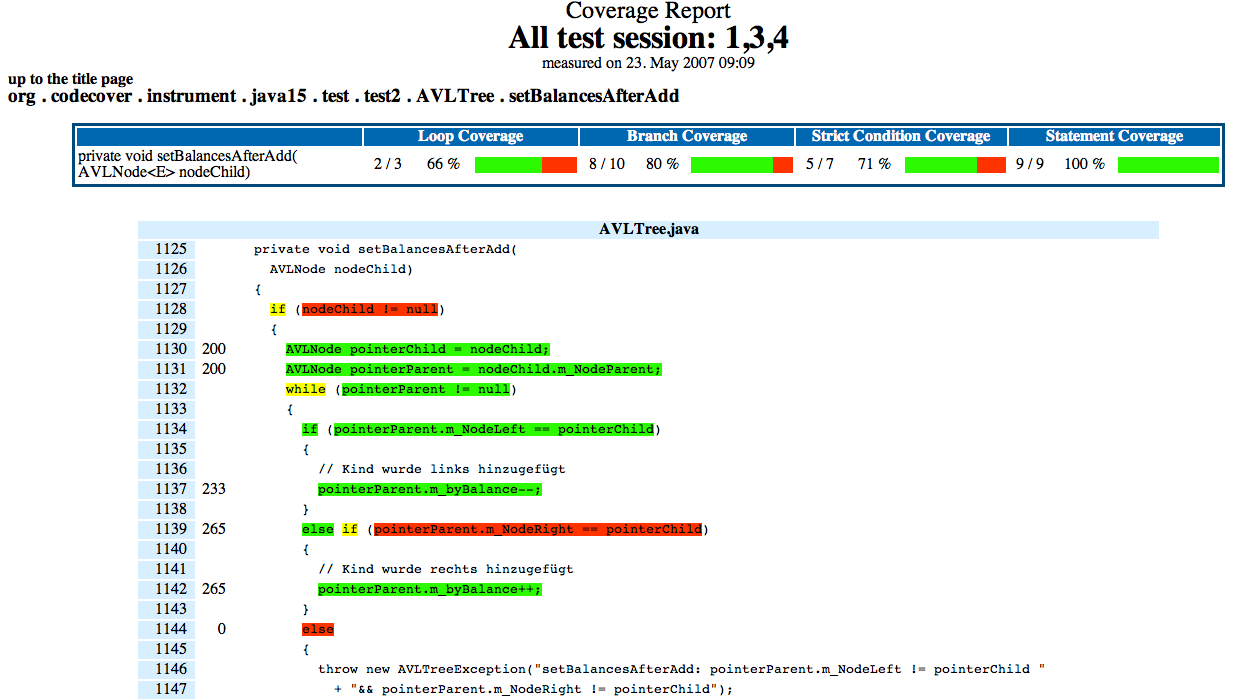
\includegraphics[width = \textwidth]{images/report_example.png}
\caption{An example CodeCover report}
\label{command:re:fig:example}
\end{center}
\end{figure}

%\end{fullpage}


%%%%%%%%%%%%%%%%%%%%%%%%%%%%%%%%%%%%%
%%%%%%%%%%%%%   Info   %%%%%%%%%%%%%%
%%%%%%%%%%%%%%%%%%%%%%%%%%%%%%%%%%%%%
\subsection{Info}\label{Command-Info}
Shows information about a test-session container. The options allow to manipulate the output, as detailed in \ref{command:info:examples}~\nameref{command:info:examples}
\subsubsection{Usage}\label{command:info:usage}
\begin{quote}
\code{codecover info [options]}
\end{quote}

\subsubsection{Options}\label{command:info:options}
\seealso{\nameref{General}}
The following table lists all the options, that are available for use with this command.\\

\begin{longtable}{|l|p{4cm}|c|}\hline
   {\textbf{Option}} & 
   {\textbf{Description}} & 
   {\textbf{Required}} \\\hline \hline \endhead
   \verb$-c, --container <file>$ & the test-session container & \x \\\hline
   \verb$-s, --session <name>$ & the name of a test-session &  \\\hline
   \verb$-t, --test-cases$ & showing test case information &  \\\hline
  \caption{Options for command info}
  \label{fr_tb:Options for command info}
\end{longtable}
\subsubsection{Examples}\label{command:info:examples}
\marginlabel{General example}
The following shows the different information levels \codecover provides. Calling the info command with only the test-session container, results in a list of all the test-session contained in this test-session container, with their name, and the date, they were created on. By naming test-sessions present in the test-session container, you can tailor the output to your specific needs.

\begin{verbatim}
root@deepthought:~> codecover info -c container.xml
---------------------------------------------------------------------
test-session container: container.xml

test-sessions:
name         | date                                        
---------------------------------------------------------------------
TestSession0 | 2007-05-18 17:47:32 +0200 (Fri, 18 May 2007)
TestSession1 | 2007-05-18 17:47:32 +0200 (Fri, 18 May 2007)
TestSession2 | 2007-05-18 17:47:32 +0200 (Fri, 18 May 2007)
---------------------------------------------------------------------	
\end{verbatim}

\marginlabel{Example with \code{verbose}}
Adding "verbose" as an option to the above call, additionally displays the comment of the test-sessions in the test-session container.

\begin{verbatim}
root@deepthought:~> codecover info --verbose
                                   -c container.xml
---------------------------------------------------------------------
test-session container: container.xml

test-sessions:
name         | date                                         | comment
---------------------------------------------------------------------
TestSession0 | 2007-05-18 17:47:32 +0200 (Fri, 18 May 2007) | 42
TestSession1 | 2007-05-18 17:47:32 +0200 (Fri, 18 May 2007) | 42
TestSession2 | 2007-05-18 17:47:32 +0200 (Fri, 18 May 2007) | 42
---------------------------------------------------------------------
\end{verbatim}

\marginlabel{Example with \code{test-cases}}
Calling the info command with the "test-cases" option results in a more detailed break-down of the test-session container. Each test-session is listed, as well as a list of all the test cases contained in it. This list of test cases provides the name of the test case and its creation date.

\begin{verbatim}
root@deepthought:~> codecover info --test-cases 
                                   -c container.xml 
                                   -s TestSession0
---------------------------------------------------------------------
test-session container: container.xml
=====================================================================
test-session name:    TestSession0
test-session date:    2007-05-18 17:47:32 +0200 (Fri, 18 May 2007)
test-session comment: 42

test cases:
name        | date                                        
---------------------------------------------------------------------
TestCase0   | 2007-05-18 17:47:32 +0200 (Fri, 18 May 2007)
TestCase99  | 2007-05-18 17:47:32 +0200 (Fri, 18 May 2007)
TestCase198 | 2007-05-18 17:47:32 +0200 (Fri, 18 May 2007)
TestCase297 | 2007-05-18 17:47:32 +0200 (Fri, 18 May 2007)
---------------------------------------------------------------------
\end{verbatim}

\marginlabel{Example with \code{test-cases} and \code{verbose}}
As before, calling the info command with "test-cases" option, as well as the "verbose" option, adds the comments to the list of test cases in the given test-session

\begin{verbatim}
root@deepthought:~> codecover info --verbose 
                                   --test-cases 
                                   -c container.xml 
                                   -s TestSession0
---------------------------------------------------------------------
test-session container: container.xml
=====================================================================
test-session name:    TestSession0
test-session date:    2007-05-18 17:47:32 +0200 (Fri, 18 May 2007)
test-session comment: 42

test cases:
name        | date                                         | comment
---------------------------------------------------------------------
TestCase0   | 2007-05-18 17:47:32 +0200 (Fri, 18 May 2007) | 42
TestCase99  | 2007-05-18 17:47:32 +0200 (Fri, 18 May 2007) | 42
TestCase198 | 2007-05-18 17:47:32 +0200 (Fri, 18 May 2007) | 42
TestCase297 | 2007-05-18 17:47:32 +0200 (Fri, 18 May 2007) | 42
---------------------------------------------------------------------
\end{verbatim}


%%%%%%%%%%%%%%%%%%%%%%%%%%%%%%%%%%%%%
%%%%%%%%%%  Merge Sessions  %%%%%%%%%
%%%%%%%%%%%%%%%%%%%%%%%%%%%%%%%%%%%%%
\subsection{Merge Sessions}\label{Command-Merge-Sessions}
This command is used to merge one or more test-sessions of a session container into a new test-session.
\subsubsection{Usage}\label{command:ms:usage}
\begin{quote}
\code{codecover (merge-sessions|ms) [options]}
\end{quote}

\subsubsection{Options}\label{command:ms:options}
\seealso{\nameref{General}}
The following table lists all the options, that are available for use with this command.
\begin{longtable}{|l|p{4cm}|c|}\hline
   {\textbf{Option}} & 
   {\textbf{Description}} & 
   {\textbf{Required}} \\\hline \hline \endhead
   \verb$-c, --container <file>$ & the session container to use & \x \\\hline
   \verb$-s, --session <name>$ & a name of a test-session participating in the merging; this argument can occur more than one time -- once for every participant & \x \\\hline
   \verb$-r, --remove-old-test-sessions$ & indicates, whether or not the test-sessions, that were merged, are removed after merging & \\\hline
   \verb$-n, --name <name>$ & the name of the merged test-session & \x \\\hline
   \verb$-m, --comment <text>$ & a comment describing the merged test-session & \\\hline
  \caption{Options for command merge-sessions}
  \label{fr_tb:Options for command merge-sessions}
\end{longtable}

\subsubsection{Examples}\label{command:ms:examples}
\begin{quote}
\begin{verbatim}
codecover merge-sessions -c container.xml 
                         -n "Merged test-session" 
                         -s "test-session 1" "test-session 2" 
\end{verbatim}
\end{quote}
Loads the test-session container from the file "container.xml" and merges the two test-sessions "test-session 1" and "test-session 2" into the new "Merged test-session". By default the merged test-sessions - "test-session 1" and "test-session 2" - are \emph{not} deleted.
\begin{quote}
\begin{verbatim}
codecover merge-sessions --remove-old-test-sessions 
                         -c container.xml 
                         -s "test-session 1" "test-session 2"
                         -n "Merged test-session" 
\end{verbatim}
\end{quote}
Adding the "remove-old-test-sessions" to the command performs the operation described above, but deletes the merged test-sessions - "test-session 1" and "test-session 2" - from the test-session container.
%%%%%%%%%%%%%%%%%%%%%%%%%%%%%%%%%%%%%
%%%%%%%%%%% Alter Session %%%%%%%%%%%
%%%%%%%%%%%%%%%%%%%%%%%%%%%%%%%%%%%%%
\subsection{Alter Session}\label{Command-Alter-Session}
This command is used to modify the name and/or the comment of a test-session.
\subsubsection{Usage}\label{command:as:usage}
\begin{quote}
\code{codecover (alter-session|as) [options]}
\end{quote}

\subsubsection{Options}\label{command:as:options}
\seealso{\nameref{General}}
The following table lists all the options, that are available for use with this command.
\begin{longtable}{|l|p{4cm}|c|}\hline
   {\textbf{Option}} & 
   {\textbf{Description}} & 
   {\textbf{Required}} \\\hline \hline \endhead
   \verb$-c, --container <file>$ & the session container to use & \x \\\hline
   \verb$-s, --session <name>$ & the old name of the test-session & \x \\\hline
   \verb$-n, --name <name>$ & a new name of the test-session & \\\hline
   \verb$-m, --comment <text>$ & a new comment describing the test-session & \\\hline
  \caption{Options for command alter-session}
  \label{fr_tb:Options for command alter-session}
\end{longtable}

\subsubsection{Examples}\label{command:as:examples}
\begin{quote}
\begin{verbatim}
codecover alter-session -c container.xml 
                        -s "Session 1"
                        -n "New Name" 
                        -m "New Comment"
\end{verbatim}
\end{quote}
Load the test-session container from "container.xml", rename the test-session with the name "Session 1" to "New Name" and change the comment of it to "New Comment". The option for the comment is not required, so a test-session can be renamed without changing its comment.

%%%%%%%%%%%%%%%%%%%%%%%%%%%%%%%%%%%%%
%%%%%%%%%%%% Copy Sessions %%%%%%%%%%
%%%%%%%%%%%%%%%%%%%%%%%%%%%%%%%%%%%%%
\subsection{Copy Sessions}\label{Command-Copy-Sessions}
This command is used to copy one or more test-sessions from one session container to another. \newline
\attention
If the destination test-session container does not exists, the source test-session container is copied to the location of the destination test-session container, while containing only the specified test-sessions.\newline
\attention
If the destination test-session container already contains a test-session, that is to be copied into it, from the source test-session container, the copied test-session is renamed along the lines of "Test Session" to "Test Session (1)". The test-session that was already present in the destination test-session container is not modified. 

\subsubsection{Usage}\label{command:cs:usage}
\begin{quote}
\code{codecover (copy-sessions|cs) [options]}
\end{quote}

\subsubsection{Options}\label{command:cs:options}
\seealso{\nameref{General}}
The following table lists all the options, that are available for use with this command.
\begin{longtable}{|l|p{4cm}|c|}\hline
   {\textbf{Option}} & 
   {\textbf{Description}} & 
   {\textbf{Required}} \\\hline \hline \endhead
   \verb$-c, --container <file>$ & the source session container & \x \\\hline
   \verb$-s, --session <name>$ & a name of a test-session participating at the copy; this argument can occur more than one time -- once for every participant & \x \\\hline
   \verb$-d, --destination <file>$ & the destination session container & \x \\\hline
  \caption{Options for command copy-sessions}
  \label{fr_tb:Options for command copy-sessions}
\end{longtable}

\subsubsection{Examples}\label{command:cs:examples}
\begin{quote}
\begin{verbatim}
codecover copy-sessions -c container.xml 
                        -s "Session 1" 
                        -s "Session 3" 
                        -d container2.xml
\end{verbatim}
\end{quote}
Load the test-session containers from "container.xml", copies the sessions named "Session 1" and "Session 3" to the test-session container from "container2.xml".
%%%%%%%%%%%%%%%%%%%%%%%%%%%%%%%%%%%%%
%%%%%%%%%% Remove Sessions %%%%%%%%%%
%%%%%%%%%%%%%%%%%%%%%%%%%%%%%%%%%%%%%
\subsection{Remove Sessions}\label{Command-Remove-Sessions}
This command is used to remove one or more test-sessions from a session container.
\subsubsection{Usage}\label{command:rs:usage}
\begin{quote}
\code{codecover (remove-sessions|rs) [options]}
\end{quote}

\subsubsection{Options}\label{command:rs:options}
\seealso{\nameref{General}}
The following table lists all the options, that are available for use with this command.
\begin{longtable}{|l|p{4cm}|c|}\hline
   {\textbf{Option}} & 
   {\textbf{Description}} & 
   {\textbf{Required}} \\\hline \hline \endhead
   \verb$-c, --container <file>$ & the session container to remove from & \x \\\hline
   \verb$-s, --session <name>$ & the name of the test-session to be removed; this argument can occur more than one time -- once for every test-session & \x \\\hline
  \caption{Options for command remove-sessions}
  \label{fr_tb:Options for command remove-sessions}
\end{longtable}

\subsubsection{Examples}\label{command:rs:examples}
\begin{quote}
\begin{verbatim}
codecover remove-sessions -c container.xml 
                          -s "Session 1"
\end{verbatim}
\end{quote}
Load the test-session container from "container.xml", remove the test-session with the name "Session 1" of the container.

%%%%%%%%%%%%%%%%%%%%%%%%%%%%%%%%%%%%%
%%%%%%%%% Merge Test Cases %%%%%%%%%%%
%%%%%%%%%%%%%%%%%%%%%%%%%%%%%%%%%%%%%
\subsection{Merge Test Cases}\label{Command-Merge-Test-Cases}
This command is used to merge one or more test-cases of a test-session into a new test-case.
\subsubsection{Usage}\label{command:mt:usage}
\begin{quote}
\code{codecover (merge-test-cases|mt) [options]}
\end{quote}

\subsubsection{Options}\label{command:mt:options}
\seealso{\nameref{General}}
The following table lists all the options, that are available for use with this command.
\begin{longtable}{|l|p{4cm}|c|}\hline
   {\textbf{Option}} & 
   {\textbf{Description}} & 
   {\textbf{Required}} \\\hline \hline \endhead
   \verb$-c, --container <file>$ & the session container to use & \x \\\hline
   \verb$-s, --session <name>$ & the name of the test-session & \x \\\hline
   \verb$-t, --test-case <name>$ & a name of a test case participating in the merging; this argument can occur more than one time -- once for every participant & \x \\\hline
   \verb$-r, --remove-old-test-cases$ & indicates, whether or not the test cases, that were merged, are removed after merging & \\\hline
   \verb$-n, --name <name>$ & the name of the merged test case & \x \\\hline
   \verb$-m, --comment <text>$ & a comment describing the merged test case & \\\hline
  \caption{Options for command merge-test-cases}
  \label{fr_tb:Options for command merge-test-cases}
\end{longtable}

\subsubsection{Examples}\label{command:mt:examples}
\begin{quote}
\begin{verbatim}
codecover merge-test-cases -c container.xml 
                           -s "Session 1"
                           -t "test-case 1" "test-case 2" 
                           -n "Merged test-case"
\end{verbatim}
\end{quote}
Loads the test-session container from the file "container.xml" and merges the two test-cases "test-case 1" and "test-case 2" into the new test-case "Merged test-case". By default the merged test-cases - "test-case 1" and "test-case 2" - are \emph{not} deleted.
\begin{quote}
\begin{verbatim}
codecover merge-test-cases --remove-old-test-cases 
                           -c container.xml 
                           -s "Session 1"
                           -t "test-case 1" "test-case 2" 
                           -n "Merged test-case"
\end{verbatim}
\end{quote}
Adding the "remove-old-test-cases" to the command performs the operation described above, but deletes the merged test-cases - "test-case 1" and "test-case 2" - from the test-session container.

%%%%%%%%%%%%%%%%%%%%%%%%%%%%%%%%%%%%%
%%%%%%%%% Alter Test Case %%%%%%%%%%
%%%%%%%%%%%%%%%%%%%%%%%%%%%%%%%%%%%%%
\subsection{Alter Test Case}\label{Command-Alter-Test-Case}
This command is used to modify the name and/or the comment of a test-case.
\subsubsection{Usage}\label{command:at:usage}
\begin{quote}
\code{codecover (alter-test-case|at) [options]}
\end{quote}

\subsubsection{Options}\label{command:at:options}
\seealso{\nameref{General}}
The following table lists all the options, that are available for use with this command.
\begin{longtable}{|l|p{4cm}|c|}\hline
   {\textbf{Option}} & 
   {\textbf{Description}} & 
   {\textbf{Required}} \\\hline \hline \endhead
   \verb$-c, --container <file>$ & the session container to use & \x \\\hline
   \verb$-s, --session <name>$ & the name of the test-session & \x \\\hline
   \verb$-t, --test-case <name>$ & the old name of the test case & \x \\\hline
   \verb$-n, --name <name>$ & the new name of the test case & \\\hline
   \verb$-m, --comment <text>$ & a new comment describing the test case & \\\hline
  \caption{Options for command alter-test-case}
  \label{fr_tb:Options for command alter-test-case}
\end{longtable}

\subsubsection{Examples}\label{command:at:examples}
\begin{quote}
\begin{verbatim}
codecover alter-test-case -c container.xml 
                          -s "Session 1"
                          -t "Test Case 1" 
                          -n "New Name" 
                          -m "New Comment"
\end{verbatim}
\end{quote}
Load the test-session container from "container.xml", rename the test-case with the name "Test Case 1" to "New Name" and change the comment of the test-case to "New Comment". The option for the comment is not required, so a test-case can be renamed without changing its comment.

%%%%%%%%%%%%%%%%%%%%%%%%%%%%%%%%%%%%%
%%%%%%%% Remove Test Cases %%%%%%%%%%
%%%%%%%%%%%%%%%%%%%%%%%%%%%%%%%%%%%%%
\subsection{Remove Test Cases}\label{Command-Remove-Test-Cases}
This command is used to remove a test-case from a test-session.
\subsubsection{Usage}\label{command:rt:usage}
\begin{quote}
\code{codecover (remove-test-cases|rt) [options]}
\end{quote}

\subsubsection{Options}\label{command:rt:options}
\seealso{\nameref{General}}
The following table lists all the options, that are available for use with this command.
\begin{longtable}{|l|p{4cm}|c|}\hline
   {\textbf{Option}} & 
   {\textbf{Description}} & 
   {\textbf{Required}} \\\hline \hline \endhead
   \verb$-c, --container <file>$ & the session container to use & \x \\\hline
   \verb$-s, --session <name>$ & the name of the test-session & \x \\\hline
   \verb$-t, --test-case <name>$ & the name of the test case to be removed; this argument can occur more than one time -- once for every test case & \x \\\hline
  \caption{Options for command remove-test-cases}
  \label{fr_tb:Options for command remove-test-cases}
\end{longtable}

\subsubsection{Examples}\label{command:rt:examples}
\begin{quote}
\begin{verbatim}
codecover remove-test-cases -c container.xml 
                            -s "Session 1"
                            -t "Test Case 1"
\end{verbatim}
\end{quote}
Load the test-session container from "container.xml", remove the test-case with the name "Test Case 1" of the session "Session 1".

%%%%%%%%%%%%%%%%%%%%%%%%%%%%%%%%%%%%%
%%%%%%%%%%     Help    %%%%%%%%%%%%%%
%%%%%%%%%%%%%%%%%%%%%%%%%%%%%%%%%%%%%
\subsection{Help}\label{Command-Help}
The help command can be used either to show a help page containing an overview of all command, or to show all information about one given command, including all options and parameters of it.
\subsubsection{Usage}\label{command:help:usage}
\begin{quote}
\code{codecover (help|h) [\%command\%]}
\end{quote}

\subsubsection{Options}\label{command:help:options}
The help command has no options.

\subsubsection{Examples} \label{command:help:examples}
\begin{quote}
\begin{verbatim}
codecover in --help
\end{verbatim}
\end{quote}
or
\begin{quote}
\begin{verbatim}
codecover h in
\end{verbatim}
\end{quote}

Show the usage, the available options and parameters of the instrument command.
The output for this command will be:

\begin{verbatim}
root@deepthought:~> codecover in --help
usage: codecover instrument [options]
instruments source files
 -r,--root-directory <directory>   the root directory of the source 
                                   files (e.g. the default package)
 -f,--selection-file <file>        a file containing a list of files or
                                   folders to instrument, they are
                                   relative to the root directory
 -V,--version                      prints the version
 -a,--charset <charset>            the charset of the code files
 -c,--container <file>             the test session container that will
                                   be created
 -d,--destination <directory>      destination directory for 
                                   instrumented code
 -h,--help                         shows help page
 -i,--criterion <crit>             one or more of (all, st, br, co, lo)
 -l,--language <lang>              e.g. java, cobol
 -o,--code <file/directory>        a file or a folder to instrument;
                                   this argument can occur more than 
                                   one time, they are relative to the
                                   root directory
 -p,--pretend                      no data changes, only simulation
 -q,--quiet                        print no information at all
 -v,--verbose                      print more information as usual
\end{verbatim}
\svnid{$Id: JavaMeasurement.tex 1 2007-12-12 17:37:26Z t-scheller $}
\section{Measurement under Java}
The following sections descibes some special features of the instrumentation and coverage measurement process under Java, if you use the Java instrumenter shipped together with \codecover.

\subsection{Test case selection}
All coverage data collected during a test run is called a test session. You can subdivide this test session into test cases. There is a number of methods to do this.
\subsubsection{One test case}
If you just instrument your classes and run it on your own, only one test case containing all coverage data will be produced. This test case has the name \textit{UNNAMED TESTCASE}.
\subsubsection{Comments}
You can use specific comments in source files, that will be instrumented. These comments will be translated to method calls during the instrumentation process. For this reason, it is important, that you place these comments at such positions in your source files, where a method call is allowed. Otherwise you will receive compiler errors.
\par
The possible comments are:
\begin{verbatim}
// startTestCase("NAME");
// startTestCase("NAME", "COMMENT");
// endTestCase();
// endTestCase("NAME");
// endTestCase("NAME", "COMMENT");
// finishTestSession();
\end{verbatim}
You have to ensure, that a comment looks exactly like one of these patterns. Otherwise a comment will be ignored.
\par
The start and end test case comments explicitly start or end a test case. The start of a test case implicitly ends a prior test case, if it has not ended yet. So two test cases can not overlap.
\par
The finish test session comment forces the coverage measurement to stop, flush all remaining coverage counters and close the log. No more coverage results will be collected after this call. You can use this method for example to finish the coverage measurement of a Java dynamic web project. Here the \code{ShutdownHook} approach of \codecover might not catch the shutdown of the server or \code{webapp}.
\subsubsection{Method calls}
If you like the method of the comments, but want to use dynamic \code{Strings} as parameters, you can use specific method calls in your own test suite. For this approach, you need to add a jar file to your class path: \\
\code{java-protocol-dummy.jar} \\
And you have to call one of the methods of the class: \\ \code{org.codecover.instrumentation.java.measurement.Protocol}.
\par
Here is an example for this approach:
\lstset{language=Java}
\begin{lstlisting}[caption=Example for the usage of the Protocol]{Protocol}
try {
  Person person = null;
  for (int i = 0; i < MAX; i++ {
    person = persons[i];
    Protocol.startTestCase(person.getName());
    person.prepare();
    person.callTestMethods();
    // throws Exception
    String result = person.checkResults();
    Protocol.endTestCase(person.getName(), result);
  }
} catch (Exception e) {
  Protocol.endTestCase(person.getName(),
    "An Exception occurred" + e.getMessage());
}
\end{lstlisting}
\subsubsection{JUnit}
\codecover supports JUnit for the test case selection too. For this approach you need not to instrument your JUnit \code{TestCases}. But you have to use so called \code{TestRunners} provided by \codecover in the jar: \\
\code{JUnit-TestRunner.jar} \\
There are a number of \code{TestRunners} available:
\begin{itemize}
  \item \code{org.codecover.junit3.swing.TestRunner}: \\
a Swing UI for JUnit 3.x
  \item \code{org.codecover.junit3.awt.TestRunner}: \\
an AWT UI for JUnit 3.x
  \item \code{org.codecover.junit3.text.TestRunner}: \\
a command line UI for JUnit 3.x
  \item \code{org.codecover.junit4.core.TestRunner}: \\
a command line UI for JUnit 4.x
\end{itemize}
These test runners can be called by:
\begin{verbatim}
java -cp junit.jar:JUnit-TestRunner.jar:bin
    org.codecover.junit.swing.TestRunner
    [-methodsAsTestCases]
    de.myprogram.AllTests
\end{verbatim}
Where \code{AllTests} is a JUnit test suite. There is an optional argument: \\ \code{-methodsAsTestCases}. \\
This tells \codecover whether to use JUnit test cases or the methods of JUnit test cases as test cases in the understanding of the software. \codecover will explicitly start end end test cases synchronously to JUnit. If there are own calls of start test case, using one of the methods described above, they might be ignored, because JUnit test cases have a higher priority.

\subsection{Coverage result}
The coverage results of a test run is stored in a so called \code{coverage log file}. Per default its file name has the following format: \\
\code{coverage-log-yyyy-MM-dd-HH-mm-ss-SSS.clf} \\
This file is stored in the current directory. To change the target of this coverage log file, you can use one of the following methods:
\begin{enumerate}
  \item System property: \\
You can set a so called system property when starting your instrumented program. The name of the property is: \\
\code{org.codecover.coverage-log-file}. \\
An example call:
\begin{verbatim}
java -Dorg.codecover.coverage-log-file=archiv/coverage1.clf
     -cp bin:library.jar
     Main
\end{verbatim}
  \item Environment variable: \\
You can set a system variable with the name: \\
\code{org.codecover.coverage-log-file}.
  \item \code{CoverageLogPath}: \\
After having instrumented your source files, additionally classes have been added. One of them is: \\
\code{org.codecover.instrumentation.java.measurement.CoverageLogPath} \\
You just can change the return value of the method \code{getDefaultPath()} to another file name or another path. Afterwards you have to recompile this class.
\end{enumerate}
If a coverage log file with the same name already exists, the name of the new \code{coverage log file} will be extended by \textit{(1)}. If you want to enable overwriting, set the following system variable to \code{"true"} or \code{"on"}: \\
\code{org.codecover.coverage-log-overwrite}. \\
Example:
\begin{verbatim}
java -Dorg.codecover.coverage-log-file=archiv/coverage2.clf
     -Dorg.codecover.coverage-log-overwrite=true
     -cp bin:library.jar
     Main
\end{verbatim}

\subsection{Special characteristics}
When instrumenting your Java source files, some additional files will be added. They lie in the following package: \\
\code{org.codecover} \\
You have to compile them and add them to your class path when executing your program, because these files are needed for the coverage measurement.
\par
The measurement approach under Java uses a so called \code{ShutdownHook}, to guarantee, that all measurement results are captured. If you use an own \code{ShutdownHook} its effected coverage data might not be captured.
\par
If you use an own \code{ClassLoader} you have to ensure, that this classloader is not instrumented because the instrumentation causes problems in this specific case.

\end{document}

%%% Local Variables:
%%% TeX-PDF-mode: t
%%% End:
